\documentclass[sigconf, timestamp-false, anonymous=true]{acmart}

\usepackage{listings}
\usepackage{multirow}
\usepackage{graphicx}
\usepackage{subcaption}
\usepackage{hyperref}
\usepackage{fancybox}
\usepackage{enumitem}


\definecolor{listinggray}{gray}{0.9}
\definecolor{lbcolor}{rgb}{0.9,0.9,0.9}
\definecolor{dkgreen}{rgb}{0,0.5,0}
\definecolor{dkred}{rgb}{0.5,0,0}
\definecolor{gray}{rgb}{0.5,0.5,0.5}
\definecolor{cyan(process)}{rgb}{0.0, 0.72, 0.92}
\definecolor{safetyorange}{rgb}{1.0, 0.4, 0.0}
\definecolor{javagreen}{rgb}{0.25,0.5,0.35}
\definecolor{metalgrey}{rgb}{0.43, 0.5, 0.5}
 % comments
%basicstyle=\ttfamily\bfseries\footnotesize,


\lstdefinestyle{JavaStyle}{
    language=Java,      % choose the language of the code
    keywords=[2]{View, LayoutInflater, ViewGroup, Bundle, ListView, Fragment, Activity},
    keywords=[3]{onCreateView, inflate, getActivity, DLE, findViewById, setAdapter},
    keywords=[4]{@Override, listView, DirList},
    basicstyle=\ttfamily\bfseries,
    keywordstyle=\color[RGB]{69,97,189},
    keywordstyle=[2]{\color{cyan(process)}},
    keywordstyle=[3]\color{javagreen},
    keywordstyle=[4]\color{metalgrey},
    %safetyorange
    commentstyle=\itshape\color{green!60!black},
    moredelim=[l][\itshape\color{gray}]{//}, %<--- overrides line-comment style
    stringstyle=\color[RGB]{192,8,8},
    numberstyle=\itshape\color{yellow!50!black},
%   backgroundcolor=\color{lbcolor},
    tabsize=4,
%   rulecolor=,
    upquote=true,
    aboveskip={1.5\baselineskip},
    columns=fixed,
    showstringspaces=false,
    extendedchars=false,
    breaklines=true,
    prebreak = \raisebox{0ex}[0ex][0ex]{\ensuremath{\hookleftarrow}},
    frame=single,
    numbers=left,
    showtabs=false,
    showspaces=false,
    showstringspaces=false,
    %autodedent,%<--- removes indentation
}
\lstset{style=JavaStyle}

%% Rights management information.  This information is sent to you
%% when you complete the rights form.  These commands have SAMPLE
%% values in them; it is your responsibility as an author to replace
%% the commands and values with those provided to you when you
%% complete the rights form.
\setcopyright{none}

\acmConference[ESEC/FSE '20]{ESEC/FSE '20: ACM Joint European Software Engineering Conference and Symposium 
on the Foundations of Software Engineering}{November 8-13, 2020}{Sacramento, CA, USA}
\acmYear{2020}

\newcommand\todo[1]{\textcolor{red}{#1}}

%%
%% Submission ID.
%% Use this when submitting an article to a sponsored event. You'll
%% receive a unique submission ID from the organizers
%% of the event, and this ID should be used as the parameter to this command.
%%\acmSubmissionID{123-A56-BU3}

%%
%% The majority of ACM publications use numbered citations and
%% references.  The command \citestyle{authoryear} switches to the
%% "author year" style.

%%
%% end of the preamble, start of the body of the document source.
\title{A Study of Multi-Location Bug Patches}
\begin{document}



%add authors & shortauthors if we are lucky :)

\begin{abstract}
    Automatic program repair is a promising approach for reducing the
    cost of quality assurance practices and faulty software. To date, most
    techniques proposed for test-driven automatic repair have succeeded
    primarily on bugs that benefit from short, single-location patches. Techniques
    that successfully generate multi-location patches often do so in an
    alternative, single-edit way, or by targeting particular multi-location bug
    patterns. Empirical studies of real-world similarly tend to focus on the
    patterns exhibited by single-location bug patches, and have not examined repairability
    of multi-location patches in detail. We present a comprehensive empirical analysis
    of multi-location patches for bugs in open source Java programs, focusing on static and
    dynamic properties that define the repair search space for a given bug.
    This analysis focuses on the key challenges of the dynamic program repair
    problem: the \emph{mutations and fix code} used to repair bugs in multiple locations;
    the \emph{fault locations} and their relationships; and the \emph{objective
      function}, and in particular how and to what degree test cases can be used
    (or not) to identify partial repairs. We identify key takeaways and
    challenges, with implications for future work in expressive, multi-location bug
    repair.
\end{abstract}

%%
%% The code below is generated by the tool at http://dl.acm.org/ccs.cfm.
%% Please copy and paste the code instead of the example below.
\begin{CCSXML}
<ccs2012>
<concept>
<concept_id>10011007.10011074.10011099.10011102</concept_id>
<concept_desc>Software and its engineering~Software defect analysis</concept_desc>
<concept_significance>500</concept_significance>
</concept>
<concept>
<concept_id>10011007.10011074.10011784</concept_id>
<concept_desc>Software and its engineering~Search-based software engineering</concept_desc>
<concept_significance>500</concept_significance>
</concept>
</ccs2012>
\end{CCSXML}

\ccsdesc[500]{Software and its engineering~Software defect analysis}
\ccsdesc[500]{Software and its engineering~Search-based software engineering}

\keywords{software bugs, program repair}

\maketitle


\newcommand{\rqorinsight}[2]{
  \setlength{\fboxsep}{0.8em}
  \vspace{0.5em}
  \begin{center}
  \Ovalbox{\begin{minipage}{0.9\linewidth}
    \textbf{RQ#1:} #2
    \end{minipage}}
  \end{center}
  \vspace{0.5em}}

\section{Introduction}

Buggy software has a significant economic cost~\cite{cambridge-study}, and
software failures are estimated to have affected half of the world's
population~\cite{tricentis}. Software, and thus buggy software, has become
ubiquitous. The increased developer workload has motivated research in
techniques to automatically find and fix bugs, which have become integrated into
real-world development: Facebook now includes automated repair in their
production
environment.\footnote{https://engineering.fb.com/developer-tools/getafix-how-facebook-tools-learn-to-fix-bugs-automatically/}

A significant class of program repair techniques in both
research~\cite{genprog,angelix,Le17, Xuan17} and practice~\cite{sapfix} use test
cases to guide patch construction, typically by following what's known as a
generate-and-validate paradigm. At a high level, these techniques use test cases
to localize a defect --- identified by at least one failing test --- to a set of
likely-suspicious program locations. Then, they use a variety of techniques to
construct (or \emph{generate}) patch candidates for the bug in question,
checking each to see (or \emph{validate}) if any of them cause the program to
pass all of the provided test cases.
%
Patches are constructed in a variety of ways, ranging from heuristic, syntactic
program manipulation~\cite{par,genprog,rsrepair,ae,prophet,hdrepair}, to specially adapted program
synthesis techniques~\cite{Konighofer11,Konighofer12,semfix,DeMarco14,angelix}. These techniques have successfully
repaired real, meaningful defects in large, complex
programs~\cite{angelix,genprog-eight-dollars,prophet,sapfix}.

Practically speaking, these techniques are typically limited in the types and
variety of defects they can repair. Often this is by design: techniques may
limit the repair search space to single-location patches for
tractability~\cite{rsrepair,ae,hdrepair}, while others only target certain
classes of bugs~\cite{Xuan17,sapfix,DeMarco14,par}. However, even techniques
that can in principle generate repairs with multi-location patches typically
don't~\cite{patch-correctness}.

This leaves a large proportion of real-world bugs unrepairable by modern
research techniques in program repair.  Over half of the bugs in the popular bug
benchmark Defects4J are patched by humans using multi-part
patches~\cite{d4j-dissection}. Approximately 70\% of buggy source files in a
large study of bugs in Apache projects required edits at two or more
locations~\cite{zhong2015}.

A key tension in the design of an automated repair technique is the balance
between giving users confidence in patch correctness by maximizing its
subjective quality while managing a trivially-infinite search space. This space
is typically parameterized along several axes: (1) the \emph{fault space}:
potential program locations to be modified, (2) the \emph{mutation space}: which
modifications may be applied at a location, and (3) the \emph{fix space}: code
that may be instantiated for a specific mutation. For example, a repair
technique might identify the location of a null-pointer dereference (exploring
the fault space), decide to insert new code (mutation space), and synthesize
code to initialize the pointer (fix space). Many dynamic repair techniques can
be compared in terms of their choices along each of these axes, and traversal
strategies have first-order implications for scalability and for the type and
quality of patches produced.

Multi-location repair poses distinct challenges for each of these axes for repair.
Spectrum-based fault localization~\cite{ochiai}, the most prevalent class of
fault localization techniques used in program repair, does not specifically
identify sets of locations that might be related or repaired together; indeed,
the evaluation of most fault localization techniques typicaly assumes that a bug
is localized if any one buggy line is identified~\cite{fl-survey-wong}.
Researchers have observed that some bugs are
repaired in multiple locations using very similar
code~\cite{saha2019harnessing,jiang2019cmsuggester}, informing novel techniques
that constrain the \emph{fix space} of possible multi-location repairs accordingly.
One key question for applicability of these types of techniques is how prevalent
such bugs are, and how often multi-location patches instead require multiple
coordinating (but ultimately different) edits or pieces of fix code.  Over 50\% of the fixes in four 
Apache projects involve two or more entities -- i.e., a Java class, method, or field -- and 66\%-76\% of 
those multi-entity fixes involved syntactic dependencies~\cite{wang2018}. 
Test cases are used to evaluate candidate repairs in virtually all dynamic
generate-and-validate repair techniques, but, anecdotally, may not be effective
at identifying partial repairs in a multi-location
context~\cite{better-fitness}.  
Although multi-location repair has been discussed in the context of other analyses
that study bug fix characteristics in general~\cite{d4j-dissection} as well as for
repair applicability specifically~\cite{zhong2015, wang2018}, to the best of our
knowledge there has been no significant previous study of the characteristics of
multi-location repairs in terms of their implications for repairability or, more
broadly, program repair.  

In this paper, we present a systematic study of real-world bugs with
multi-location patches,
looking specifically at their characteristics with respect to the problem of the
automatic repair search space.  
We study the bugs curated in two
real-world datasets that support program repair research: Defects4J~\cite{defects4j}
and BEARS~\cite{bears}, in total, 578 bugs in 40 projects. 
More than half of these bugs were repaired by a
human developer using edits at multiple locations.  We look at characteristics along each of the
relevant axes of the program repair search problem: fault locations, mutation
operators, fix code, and evaluation (or fitness or objective) using test cases.  Our 
contributions are
as follows:\footnote{We will complete the presentation of our replication package post review, as an additional contribution.}

\begin{itemize}
\item An analysis and enumeration of multi-location patches in Defects4J and Bears.
\item \textbf{Fault Localization.}  We find that 58\% of relevant bugs have faulty locations that are not
  covered by all failing tests, thus the assumptions underlying spectrum-based
  fault localization may not necessarily hold when used off-the-shelf for
  multi-location repair.
\item \textbf{Edit dependency.} We 
find that half of bug patches contain dependent edits, and that bugs with dependent 
edits in their patches may be more difficult to automatically repair.
\item \textbf{Cloning in multi-location repair} We find that over 30\% of bugs with multi-location
patches have very similar edits applied to different locations, suggesting the viability of 
program repair techniques designed to utilize code clones. Moreover, bugs in which 
none of the faulty locations are covered by all failing tests tend to have code clones, 
suggesting a way to tell when we should use a program repair technique designed for code 
clones.
\item \textbf{Test cases for patch validation.} We find that over 40\% of bugs with multi-location
  patches in Defects4j more than half in Bears do not require the edits at every
  location in their provided human patches to pass all test cases, suggesting
  that either patches contain unecessary edits or (more likely) that test cases
  do not fully capture the desired behavioral specification.  We also find that test 
  case based validation methods can positively identify close to 40\% of partial repairs,
  while less than
  17\% of partial repairs cause more test assertions to fail. Additionally, the 
  \emph{granularity} at which test suite behavior is measured (i.e., at the class,
  method, or assertion level) influences ability to identify partial
  repairs. 
\end{itemize}

% In Section~\ref{sec:background}, we provide background on
% generate-and-validate program repair, with a focus on the key parameters of the
% program repair search; outline our definition of a multi-edit repair for the
% purposes of this study; and outline our research questions.  We overview the key
% characteristics of the datasets that we use in our study in
% Section~\ref{sec:data-rq1}.  We then describe the results of our study along
% three key axes of program repair: fault localization (Section~\ref{secFL}),
% mutation operators and fix code (Section~\ref{sec:mutops}), and test cases as
% the patch validation mechanism (Section~\ref{sec:tests}).  We conclude by
% outlining limitations (Section~\ref{sec:limits}), related work
% (Section~\ref{sec:related}), and summarizing discussion  (Section~\ref{sec:conclusions}).

\section{Key Terms and Concepts}
\label{sec:background}

\paragraph{Search spaces in automatic program repair.} Automatic program repair (APR) techniques aim to find patches for bugs in
programs.  We restrict attention to dynamic or test-case guided program repair,
which describes the majority of research advancements over the past ten years.
Such techniques take as input a program and a set of test cases that serve as
the oracle for program correctness.  At least one of those tests should be
failing, corresponding to the bug to be repaired.

At a high level, any APR technique aims to solve a search or optimization
problem, seeking a set of edits (or patch) to the program that will lead it to
pass all of the provided tests. The repair search space is typically defined
along the following axes~\cite{ae,sqjo}:
\begin{itemize}

\item \emph{Fault space.} The first problem in fixing a bug concerns
  \emph{where} in the code modifications should be applied. Dynamic repair
  techniques begin by using test cases as input to a fault localization
  technique. Such techniques identify (and typically score) suspicious code
  based on which test cases execute which pieces of code. Although the
  particulars of the fault localization employed can vary, most APR techniques use some
  variant of spectrum-based fault localization (SBFL)~\cite{ochiai} in this first
  step. The resulting computation defines the fault space, or the candidate
  locations or code entities considered for repair.

\item \emph{Mutation space.} The mutation space is the set of applicable
  modifications at a given program location. Examples include GenProg's
  \emph{append}, \emph{replace}, and \emph{delete} mutation operators over
  statements~\cite{genprog-operators}; Par's human patch inspired edit
  templates~\cite{par} and Nopol's condition replacement over 
  \texttt{if} statements and missing precondition addition over non-branch and
  non-loop statements~\cite{Xuan17}.  A larger mutation space generates a richer
  search space with potentially more repairs, but increases its size
  combinatorially~\cite{long-search-spaces}.

\item \emph{Fix space.} Often, given a selected mutation, code must be generated
  or selected to instantiate the mutation in question.  For example, if a
  technique elects to insert a null
  pointer check, the object being checked for null must be selected to
  instantiate the templated repair from suitable variables at the code location;
  if a technique choose to insert a new piece of code at a location, suitable
  code must be generated or selected for insertion. Some APR
  techniques tackle the resultant explosion of this fix space by taking
  advantage of the \emph{plastic surgery hypothesis}~\cite{plastic}, which
  assumes that a bug can be repaired by code available in other parts of the
  same program.  Learning-based approaches, by contrast, can learn models of
  code or repairs to inform modifications~\cite{prophet}; synthesis-based
  approaches constrain the synthesis engine to a small vocabulary of fix
  ingredients, possibly informed by the code near the selected faulty
  location~\cite{angelix,s3}. 

\item \emph{Validation.} Candidate patches are typically validated using the
  provided test cases as the objective function.  In an evolutionary or
  search-based context, test cases can also be used as the fitness
  function~\cite{genprog}; techniques have supplemented the test
  case objective with partial correctness measures like program
  invariants~\cite{dinglyu}, memory snapshots~\cite{source-code-checkpoint}, or
  similarity to human edits~\cite{hdrepair}, with maximization of tests passed
  maintained as one of possibly many objectives.  In a multi-edit context,
  ideally, multiple tests would be able to idnetify partial repairs that could
  be composed.  However, evidence suggests that this does not always
  apply~\cite{better-fitness,schulte}. 
\end{itemize}



\paragraph{Multi-location bugs.} There are several plausible definitions of multi- vs. single-location bugs, with
implications for how they are studied. For the purpose of this study, we define
a \emph{patch location} as a contiguous sequence of edited lines of
code.  We combine two locations if one simply opens or closes a syntactic block
inserted by the other. That is, conceptually:
\begin{lstlisting}
+ Some_edit {
+ New code
  Existing code 
+}
\end{lstlisting}
is treated as a single-location edit in our study.  We ignore changes to
comments, whitespace, or import statements. 

Although alternative definitions may have bearing on our results, we believe this is an intuitive definition consistent with the general APR paradigm.Moreover, our aim is to understand properties of 
complex bugs for the purposes of understanding the limitations of
existing repair techniques, and key future directions to
adapting or extending them to improve expressivity. 

\paragraph{Research questions.}  The parameterization of the program repair
search problems into multiple subspaces informs our empirical study of those
spaces for the purposes of understanding multi-edit repair.  We address the
following research questions:

\begin{enumerate}[label=RQ\arabic*:]
\item \emph{How prevalent are multi-location human patches are in Defects4J and Bears?}
\item \emph{Do failing tests cover different portions of the fault?}
\item \emph{How prevalent are dependencies between edited code?}
\item \emph{How often do code clones occur in bugs with multi-location
  patches? Is the existence of code clones in human patches correlated with specific
  patterns of fault localization?}
\item \emph{How often are multi-location bugs minimal with respect to their provided test cases?}
\item \emph{How well do test case based validation methods identify partial repairs?}

\end{enumerate}

\section{Dataset Characteristics}
\label{sec:data-rq1}

\begin{table*}
\begin{center}
\begin{tabular}{l | rrr  | rr | rr | rr}
\toprule
\multicolumn{10}{c}{\textbf{Defects4J}} \\
\midrule
Project & Bugs & Src (kloc) & Test (kloc) & \multicolumn{2}{c}{Multi-location} 
		& \multicolumn{2}{c}{Multi-test} & \multicolumn{2}{c}{Multi-location \&}\\
&&&&\multicolumn{2}{c}{bugs}&\multicolumn{2}{c}{bugs}&\multicolumn{2}{c}{Multi-test bugs}\\
\midrule
JFreeChart  & 26 & 193.3 & 74.6  & 11 & 42\% & 10 & 38\% & 7 & 27\%\\
Closure compiler & 133 & 150.6 & 112.6 & 55 & 41\% & 58 & 44\% & 31 & 23\%\\
Apache commons-lang & 65 & 57.8 & 47.4  & 32 & 49\% & 17 & 26\% & 13 & 20\%\\
Apache commons-math & 106 & 45.0 & 41.5 & 53 & 50\% & 28 & 26\% & 22 & 21\%\\
Mockito & 38 & 23.0 & 28.5 & 16 & 42\% & 18 & 47\% & 8 & 21\%\\
Joda-Time & 27 & 82.9 & 70.4 & 17 & 63\% & 13 & 48\% & 9 & 33\%\\
\midrule
All (Defects4J) & 395 & 552.6 & 375.0 & 184 & 47\% & 144 & 36\% & 90 & 23\%\\
\midrule
\multicolumn{10}{c}{\textbf{Bears (single-module)}} \\
\midrule
FasterXML-jackson-databind & 26 & 95.7 & 53.6 & 17 & 65\% & 4 & 15\% & 2 & 8\%\\
INRIA-Spoon & 62 & 66.2 & 30.8  & 39 & 63\% & 23 & 37\% & 18 & 29\%\\
spring-data-commons & 15 & 45.8 & 28.8  & 9 & 60\% & 6 & 40\% & 2 & 13\%\\
traccar-traccar & 42 & 47.9 & 8.6 & 24 & 57\% & 3 & 7\% & 2 & 5\%\\
30 other projects & 38 & - & - & 22 & 58\% & 36 & 95\% & 9 & 24\%\\
\midrule
All (Bears) & 183 & >255.6 & >121.8 & 111 & 61\% & 72 & 39\% & 33 & 18\% \\
\midrule
Combined (Defects4J \& Bears) & 578 & >808.2 & >496.8 & 295 & 51\% & 216 & 37\% & 123 & 21\%\\
\bottomrule
\end{tabular}
\end{center}
\caption{\label{tab:dataset-characteristics} Characteristics of the Defects4J (top) and Bears (bottom) datasets.}
\end{table*}

Our study requires a dataset of indicative, real-world,
multi-location defects.  We study both the defects in
Defects4J~\cite{defects4j} and Bears~\cite{bears}.  Table~\ref{tab:dataset-characteristics}
summarizes these datasets, both of which
consist of historical
bugs found in real world software projects. Defects4J contains 395 bugs from 
six Java software projects, and is a popular dataset for evaluating 
program repair tools that target Java~\cite{durieux-repair-them-all}.
The dataset's patches are manually minimized to isolate the bug fix 
and exclude non-repair edits such as refactorings and feature additions.

With any dataset, however, there is a risk associated that tools may overfit
to the defects in question, and there is evidence that this situation applies to
program repair and Defects4J~\cite{durieux-repair-them-all}. 
We thus also study bugs from Bears~\cite{bears}, 
a set of Java bugs derived from failed Travis-CI builds of GitHub projects. 
Bears offers 251 bugs from 72 software projects, providing a greater diversity of 
projects compared to Defects4J. 
Several projects in Bears, however, are structured as multi-module projects, 
which are not currently compatible with our automation tools.
We thus limit our analysis of Bears to 183 bugs from 34 single-module projects.


We start our analysis of multi-location patches by asking the following research question:
\rqorinsight{1}{How prevalent are multi-location human patches are in Defects4J and Bears?}

Table~\ref{tab:dataset-characteristics} lists the numbers and percentages of
multi-location patches in Defects4J and Bears. 
We find that multi-location patches comprise over half of Bears and almost half of Defects4J.
Although a multi-location human patch for a bug does not imply the 
non-existence of a simpler patch, the high proportion of bugs that have 
multi-location patches demonstrates the relevance of such bugs to fault localization and
program repair. 

Bears contains a greater proportion of 
multi-location patches compared to Defects4J. This may be the 
result of manual patch minimization in Defects4J~\cite{defects4j} 
and lack thereof in Bears.
Thus, some Bears patches may be multi-location as a result of additional 
changes added for non-repair reasons.


\section{Fault localization}

%% what are the claims, what are we studying, why are we studying it


Spectrum-based fault localization (SBFL) is the most commonly studied, as well as the most 
effective~\cite{zou2019empirical}, fault localization technique. It is a key
first step to characterizing the \emph{fault space} in automatic program repair,
narrowing the search space to a portion of the program more likely (based on
test case behavior) to correspond to the fault.  

\paragraph{SBFL Basics.} \todo{Serena, please add an explanation of how SBFL
  works; it's key to understanding the underlying assumption.  This should
  include references as appropriate.}

Given these basics, fundamentally, a core
assumption underlying SBFL is that \emph{failing tests execute buggy portions of 
the code relatively more often than passing tests.} Thus, if all failing tests execute a 
particular line of code, then that line of code is scored as more suspicious.
This assumption is well-suited to single edit repair. Indeed, the evaluation
of most SBFL techniques asks exactly the question of interest when considering a
technique's suitability for single-edit repair: how often does a given technique
correctly, highly rank individual buggy lines of code? 

Such evaluations, by and large, do not consider the implications of
suspeciousness scoring in a multi-edit repair context.  Instead, evaluations
typically consider a technique ``successful'' if it identifies \emph{any} of a
set of changed lines as highly-ranked or likely-suspicious.  While appropriate
for the question being asked in such evaluations, this does not address
suitability for multi-line program repair.  Identifying one of several buggy
locations is generally inadequate in a context where multiple locations must be
modified.  

Thus, in this research question, we investigate how well the SBFL assumption
applies to tests that identify multi-line bugs. We focus especially on
multi-line bugs that are associated with multiple tests; \todo{short explanation
  of the intuition why. This is a placeholder, I'm a bit tired and so this
  succinct explanation is escaping me.} If multiple tests all cover the multiple
modified locations well, then SBFL's core assumption holds and multi-edit repair
can expect to effectively make use of the off-the-shelf ranking these techniques
currently provide (indeed, this has been tried~\cite{angelix}). If not---that
is, if multiple tests exercise \emph{different} portions of the buggy
code---SBFL off-the-shelf will by definition be less effective in guiding APR to
correctly modifying multiple buggy locations at once.

Therefore, for multi-edit bugs with multiple identifying failing tests, do the 
different failing tests cover exactly the same patch locations, exactly 
disjoint path locations, or some combination?


\rqorinsight[2]{How well do multiple tests cover the multiple locations
  implicated in multi-edit bugs?}

\paragraph{Methodology}

Between both datasets, there are 60 total bugs that are both multi-edit and 
multi-test -- 45 in Defects4J and 15 in Bears. For each of these bugs, we used 
Jacoco to determine which of the chunks in the human patch were executed by each failing test. Using 
this coverage data, we categorized the bug as one of 
three coverage patterns: \textit{disjoint} for bugs in which no chunk is covered by all failing tests, 
\textit{same} for bugs in which all 
tests cover the exact same chunks of the patch, and \textit{overlap} for all 
other bugs, where some chunks are covered by all failing tests, but some chunks are only covered by a 
subset of failing tests.

\paragraph{Results}
The overall distribution is seen in Figure \ref{fig:coverage-all}. Over a third 
of the bugs were classified as disjoint, indicating that for a significant 
portion of bugs, the failing tests do not all execute any portion of the faulty 
code. In addition, another 22\% were classified as overlap. Thus, over half of 
the bugs that were both multi-edit and multi-test contained chunks that were 
not executed by all failing test cases.
2

\begin{figure}
	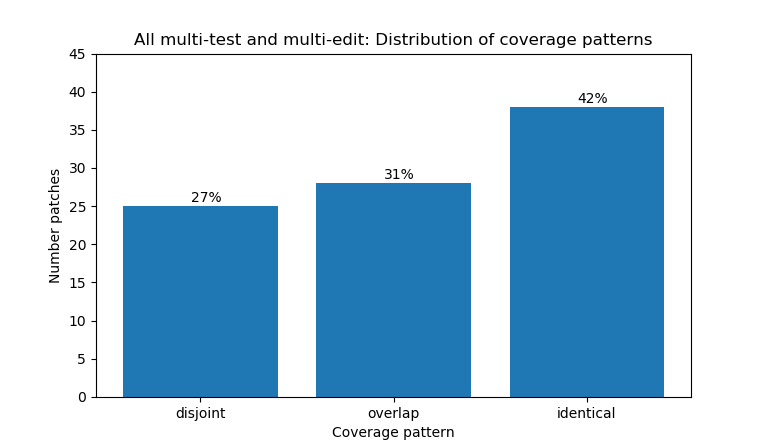
\includegraphics[width=\linewidth]{img/coverage-all.png}
	\caption{Distribution of coverage patterns for all multi-test and 
	multi-edit bugs in Bears and Defects4J. In all, 38\% of bugs were classified as disjoint, 40\% were 
	classified as same, and 22\% were classified as overlap.}
	\label{fig:coverage-all}
\end{figure}

SBFL assumes that faulty locations are executed more often by identifying 
or failing test cases and is not designed to find faults like these. Since SBFL 
is the most common fault localization technique in APR, most APR techniques 
are not well suited to fix a majority of these multi-edit and multi-test 
bugs.

If we divide distribution by dataset, we can see even more interesting 
behavior. Figure \ref{fig:coverage-datasets} shows the Defects4J dataset and 
the Bears dataset have very different distributions with respect to the 
disjoint and same categories -- in Defects4J, 47\% of bugs are disjoint and 
31\% are same, whereas in Bears, the proportions are 13\% disjoint and 67\% 
same. We hypothesize that this may be due to differences in how the two 
datasets were minimized, since Defects4J is a dataset of minimized and curated 
bugs while the bugs in Bears are taken scraped directly from the commits.


\begin{figure}
	\begin{subfigure}{\linewidth}
		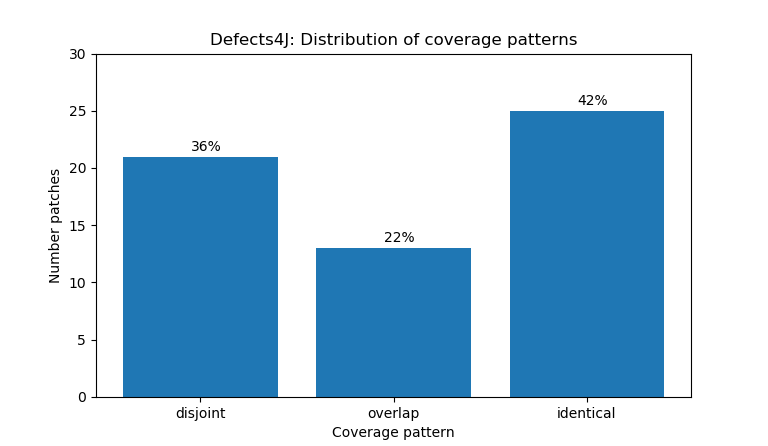
\includegraphics[width=\linewidth]{img/coverage-d4j.png}
		\caption{Distribution of coverage patterns for Defects4J. 47\% disjoint, 31\% same, and 22\% 
		overlap.}
	\end{subfigure}
	\begin{subfigure}{\linewidth}
		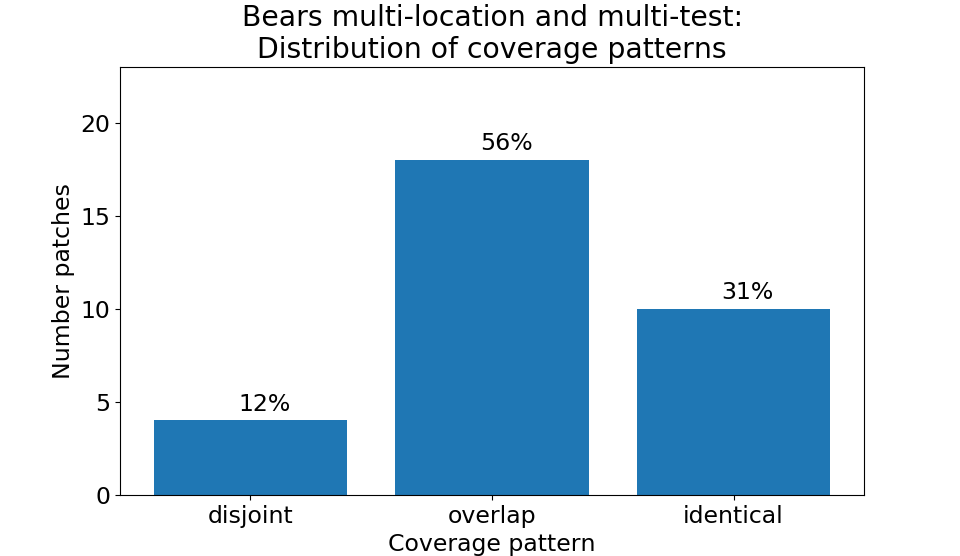
\includegraphics[width=\linewidth]{img/coverage-bears.png}
		\caption{Distribution of coverage patterns for Defects4J. 13\% disjoint, 67\% same, and 20\% 
		overlap.}
	\end{subfigure}
	\caption{Distribution of coverage patterns divided by dataset.}
	\label{fig:coverage-datasets}
\end{figure}


%\section{Symptoms}

We want to study symptoms in the context of fault localization. We define symptoms as the output given in failing test cases. In Java, most of these symptoms will be exceptions and their accompanying error message. Since most program repair is based off of failing tests, we want to see if those symptoms exhibited in those tests can correlate to type of repair.

For this paper, we specifically wanted to look at whether symptoms correlated with whether a bug could be fixed in a single location or multiple locations. If we can classify which bugs are single edit or multi edit, we can choose fault localization or patch generation techniques that are more suited.

We looked at all symptoms for all bugs in Defects4J and Bears, and categorized them based on whether they were one of the identified multi-chunk bugs or not. Then we fit the data to a linear regression model to see if there were statistically significant differences between the type of symptoms for multi edit and single edit bugs.

In order to find statistical significance, we needed to categorize the symptoms in big enough categories. We experimented with three groupings:

\begin{enumerate}
	\item Group all exceptions together except for assertion exceptions and exceptions for which a message indicates some sort of assertion (in our case, we simply looked for the keyword "expected"). We grouped the assertions into a few different types: 
	\begin{itemize}
		\item \lstinline{assert_null} is when the assertion is either expecting null, or got null when it wasn't expecting it.
		\item \lstinline{assert_int} is when the failing assertion was expecting a particular int value.
		\item \lstinline{assert_float} is the same as above, but for floats.
		\item \lstinline{assert_obj_arr_date} is when the assertion is expecting an object address, array of objects, or date object/date string. These are grouped together as commonly found but more complex assertions.
		\item \lstinline{error_expected} is when the failing test expected an exception, error, or warning.
		\item \lstinline{timeout} is when a Junit test times out, but also includes errors like stack overflows or out of memory exceptions.
		\item \lstinline{other_assert} for any other assertion that I couldn't easily categorize or parse. The large bulk of bugs in this category are bugs that had no error message at all; it simply failed with an \lstinline{AssertionError} or \lstinline{StackOverflow}.
		\item \lstinline{other}: all non-assertion exceptions.
	\end{itemize}
	\item Grouping symptoms together in an ad hoc way \todo{sell it better.}
	\begin{itemize}
		\item \lstinline{assert_prim}: assertions that compare to a Java primitive, such as int, float, or boolean.
		\item \lstinline{assert_null}: either expected or actual is null
		\item \lstinline{other_assert}: Asserting to anything that's not clearly a primitive or null.
		\item \lstinline{access}: all the bugs pertaining to wrongfully accessing or invoking certain fields or methods, or problems with classpath.
		\item \lstinline{null_pointer}: null pointer exceptions.
		\item \lstinline{timeout}: when a Junit test times out, but also includes errors like stack overflows or out of memory exceptions.
		\item \lstinline{parsing}: Anything related to parsing, serialization, or type conversion.
		\item \lstinline{other}: everything else
	\end{itemize}
	\item This last grouping is an even coarser version of the previous grouping.
	\begin{itemize}
		\item \lstinline{assert_equal}: Any assertion in which the test expected one value but got another
		\item \lstinline{other_assert}: any other assertion
		\item \lstinline{access}: all the bugs pertaining to wrongfully accessing or invoking certain fields or methods, or problems with classpath.
		\item \lstinline{null_pointer}: null pointer exceptions.
		\item \lstinline{parsing}: Anything related to parsing, serialization, or type conversion.
		\item \lstinline{other}: everything else
	\end{itemize}
\end{enumerate}

\todo{raw data from bogdan:}

assert only
\begin{lstlisting}
Call:
glm(formula = multi ~ assert_obj_arr_date + assert_int + assert_float + 
error_expected + timeout + assert_null + other_assert + other, 
family = "binomial", data = symptoms)Deviance Residuals: 
Min       1Q   Median       3Q      Max  
-1.2466  -0.5686  -0.4691  -0.4394   2.2880  Coefficients:
Estimate Std. Error z value Pr(>|z|)    
(Intercept)             -2.37550    0.38061  -6.241 4.34e-10 ***
assert_obj_arr_dateTRUE  1.24082    0.50907   2.437   0.0148 *  
assert_intTRUE           0.08619    0.45621   0.189   0.8502    
assert_floatTRUE         2.31273    0.48580   4.761 1.93e-06 ***
error_expectedTRUE       0.36735    0.53943   0.681   0.4959    
timeoutTRUE              0.99295    0.65378   1.519   0.1288    
assert_nullTRUE         -0.16611    0.58071  -0.286   0.7748    
other_assertTRUE         0.22402    0.36136   0.620   0.5353    
otherTRUE                0.63507    0.38201   1.662   0.0964 .  
---
Signif. codes:  0 '***' 0.001 '**' 0.01 '*' 0.05 '.' 0.1 ‘ ’ 1(Dispersion parameter for binomial family taken to be 1)    Null deviance: 546.49  on 645  degrees of freedom
Residual deviance: 510.11  on 637  degrees of freedom
AIC: 528.11Number of Fisher Scoring iterations: 5
\end{lstlisting}

grouping 1
\begin{lstlisting}
Call:
glm(formula = multi ~ access + assert_prim + null_pointer + timeout + 
assert_null + parsing + other_assert + other, family = "binomial", 
data = symptoms)Deviance Residuals: 
Min       1Q   Median       3Q      Max  
-0.9771  -0.6792  -0.5070  -0.4031   2.5944  Coefficients:
Estimate Std. Error z value Pr(>|z|)    
(Intercept)      -1.94778    0.36198  -5.381 7.41e-08 ***
accessTRUE        0.62756    0.41197   1.523   0.1277    
assert_primTRUE   0.81567    0.36223   2.252   0.0243 *  
null_pointerTRUE  0.32833    0.52496   0.625   0.5317    
timeoutTRUE       0.64782    0.63743   1.016   0.3095    
assert_nullTRUE  -0.52160    0.57971  -0.900   0.3682    
parsingTRUE       0.64081    0.50451   1.270   0.2040    
other_assertTRUE -0.03905    0.34777  -0.112   0.9106    
otherTRUE        -1.38263    0.76326  -1.811   0.0701 .  
---
Signif. codes:  0 '***' 0.001 '**' 0.01 '*' 0.05 '.' 0.1 ‘ ’ 1(Dispersion parameter for binomial family taken to be 1)    Null deviance: 546.49  on 645  degrees of freedom
Residual deviance: 523.84  on 637  degrees of freedom
AIC: 541.84Number of Fisher Scoring iterations: 5
\end{lstlisting}

grouping 2
\begin{lstlisting}
Call:
glm(formula = multi ~ assert_equal + access + null_pointer + 
parsing + other_assert + other, family = "binomial", data = symptoms)Deviance Residuals: 
Min       1Q   Median       3Q      Max  
-0.9390  -0.6809  -0.4377  -0.4377   2.2494  Coefficients:
Estimate Std. Error z value Pr(>|z|)    
(Intercept)       -2.0821     0.3470  -6.001 1.96e-09 ***
assert_equalTRUE   0.7532     0.3333   2.260   0.0238 *  
accessTRUE         0.7259     0.3979   1.824   0.0681 .  
null_pointerTRUE   0.4338     0.5131   0.845   0.3979    
parsingTRUE        0.7385     0.4976   1.484   0.1378    
other_assertTRUE  -0.2150     0.3223  -0.667   0.5048    
otherTRUE         -0.3646     0.5068  -0.719   0.4719    
---
Signif. codes:  0 '***' 0.001 '**' 0.01 '*' 0.05 '.' 0.1 ‘ ’ 1(Dispersion parameter for binomial family taken to be 1)    Null deviance: 546.49  on 645  degrees of freedom
Residual deviance: 527.48  on 639  degrees of freedom
AIC: 541.48Number of Fisher Scoring iterations: 5
\end{lstlisting}

In assert only, \lstinline{assert_float} correlates strongly with multiedit bugs. However, all the instances of \lstinline{assert_float} as a symptom occur in the Math package for Defects4J, and they all somehow to be multichunk. The sampling of \lstinline{assert_float} can be seenin the other two groupings as well, where \lstinline{asset_prim} and \lstinline{assert_equal}, both of which subsume \lstinline{assert_float}, are both more likey to be multi-edit.  \todo{take out math, redo analysis?}







\section{Mutation Operators and Fix Code}
\label{sec:mutops}

Given suitably selected fault locations, APR techniques vary in the types of
mutation operators they consider, how they select between them, and how they
select new fix code to instantiate them, as necessary.  For example, a na{\"i}ve
approach with only \texttt{insert}, \texttt{replace}, and \texttt{delete}
operators must choose between them at a location and, in the case of
\texttt{insert} and \texttt{replace}, choose code to insert/replace at that
location.  
%
The few techniques that handle or at least enable multi-edit patches vary in their
handling of mutation operator selection and instantiation.  At one
extreme, semantics-based repair~\cite{s3,angelix} can represent dependent edits between multiple
locations as a conjunction of multiple constraints to simultaneously solve,
bounded by some number of edits that are computationally feasible, while
restricted to a relatively small library of possible code components for use in
the inductive synthesis problem.    At the other extreme, search-based or
evolutionary techniques~\cite{genprog,par} typically treat different mutation
operators independently.  That is, a modification in one location does not
inform the selection of a modifications to apply in a second location; instead,
the heuristic search is trusted to identify copacetic combinations.  The size of
the search space increases combinatorially in this context, however, rendering
the chances of finding suitable multi-edit repairs without additional guidance
quite low~\cite{ae,long-search-spaces}. Accordingly, heuristic techniques targeted at multi-edit
repair contexts~\cite{saha2019harnessing} make assumptions about the
shape of the search space to render it tractably constrained --- in particular,
targeting bugs that can be repaired by multiple syntactically similar pieces of
fix code.

These kinds of targeted techniques surface general questions about the
\emph{relationship} between multiple edits, with implications for how edits
should be designed for automatic multi-location repair. 

\subsection{Dependencies}

One of the dimensions of the relationship between multi-location patches is potential
\emph{dependency} between the edits. Specifically, we ask the following research question:
\rqorinsight{3}{How prevalent are dependencies between edited code?}

To answer this question, we broaden the scope of multi-location patches to 
include all patches containing at least two added, removed, or modified lines, 
ignoring edits to comments, whitespace, or imports.
This expanded dataset contains 659 Defects4J v2 and 151 Bears bugs.
We consider a patch to contain dependent edits if there exists 
control or data dependencies between added, deleted, or modified statements.
We analyze deleted/modified statements in the pre-patch code 
and added/modified statements in the post-patch code for dependencies.
  
For practical performance and scalability reasons, 
we perform intraprocedural analysis. 
We do, however, gather some interprocedural data dependency information 
using the following heuristics:
\begin{itemize}
	\item If a statement invokes a method, then we assume that
	the statement reads all variables used in the method arguments.
	\item If a statement invokes a getter method \texttt{Class.getX()} 
	(for any \texttt{Class} and \texttt{X}), then we heuristically 
	assume that the statement reads \texttt{Class.X}. 
	Note that \texttt{Class.X} does not need to actually exist.
	\item If a statement invokes a setter method \texttt{Class.setX()}, 
	then we heuristically assume that the statement writes to \texttt{Class.X}. 
\end{itemize}

\paragraph{Results}

We find that 40\% of Defects4J patches, 63\% of Bears patches, 
and 45\% of the combined datasets' patches contain dependencies 
between edited statements.
Our finding supports earlier results on edit dependencies in 
bug patches~\cite{zhong2015}.
Patches with and without edit dependencies both form a substantial
portion of multi-line patches,
and neither type of patches should be ignored.

\begin{table}
{\begin{center}
	\begin{tabular}{l  rr  rr  rr}
		\toprule
		\multicolumn{7}{c}{\textbf{Patches with Dependent Edits}} \\
		\midrule
		APR (RepairThemAll) & \multicolumn{2}{c}{Defects4J} & \multicolumn{2}{c}{Bears} & \multicolumn{2}{c}{Combined} \\
		\midrule
		Success by any tool & 43 & 32\% & 9 & 9\% & 52 & 23\% \\
		Failure by all tools & 93 & 68\% & 86 & 91\% & 179 & 77 \% \\
		Not evaluated & 130 & --- & 0 & --- & 130 & --- \\
		\midrule
		Total evaluated & 136 & 100\% & 95 & 100\% & 231 & 100\% \\
		Total & 266 & --- & 95 & --- & 361 & --- \\
		\midrule
		\multicolumn{7}{c}{\textbf{Patches without Dependent Edits}} \\
		\midrule
		Success by any tool & 96 & 57\% & 7 & 13\% & 103 & 46\% \\
		Failure by all tools & 73 & 43\% & 49 & 87\% & 122 & 54\% \\
		Not evaluated & 224 & --- & 0 & --- & 224 & --- \\
		\midrule
		Total evaluated & 169 & 100\% & 56 & 100\% & 225 & 100\% \\
		Total & 393 & --- & 56 & --- & 449 & --- \\
		\bottomrule
	\end{tabular}
 \end{center}
}
	\caption{Multi-line patches with respect to the presence of 
	dependent edits and whether any APR tool successfully 
	repaired the bug in RepairThemAll~\cite{durieux-repair-them-all}.
	Bugs categorized as {\normalfont Not evaluated} are those introduced in 
	v2 of Defects4J, which RepairThemAll didn't study.}
	\label{tab:dependency-repair-contingency-table}
\end{table}

We further compare how often APR techniques 
successfully repair bugs whose patches do (not) contain edit dependencies.
Table~\ref{tab:dependency-repair-contingency-table}
show the frequencies and percentages of multi-line patches with respect to edit dependency 
and whether an APR tool successfully repaired bug in 
RepairThemAll~\cite{durieux-repair-them-all}, a repair experiment running 
11 APR tools on 5 benchmarks, including Defects4J v1 (containing a subset of Defects4J v2) and Bears.

We find that the presence of edit dependencies 
reduces the likelihood of APR tool success for Defects4J bugs.
Using a $\chi^2$ test, we find a statistically significant relationship ($p < 0.001$)
between APR success and the presence of edit dependencies for Defects4J patches. 
We fail to find statistically 
significant relationships over Bears patches, likely due to the small number (16) of 
successfully auto-repaired Bears bugs with multi-line human patches.
The generally lower auto-repairability of bugs with edit dependent patches compared 
to their non-edit dependent brethren suggest that such dependencies indeed 
add complexity to the search for a repair.

Our results substantiate prior research~\cite{zhong2015} on the frequency of 
bugs with dependent edits in human patches. A diverse range of APR 
techniques are less likely to repair such bugs. Dependent edits, however, may 
be an opportunity to constrain the search space by creating constraints between 
otherwise independent mutations. There is an opportunity to profit from edit 
dependencies to repair a large class of difficult bugs.


\subsection{Cloned code}

In addition to dependency, multi-location patches can be related through syntactic
similarity. That is, a patch can consist of a code edit applied repeatedly in
multiple locations. Thus, we ask the following research question:

\rqorinsight{4}{How often do code clones occur in multi-location bugs? Is the existence of 
	code
	clones in human patches correlated with specific patterns of fault localization?}

Previous work~\cite{wang2018} suggests that one potential fruitful way to enhance
APR techniques is to allow them to apply a single edit to multiple locations.
This is based on the observation that human developers tend to make exactly the 
same edits in multiple locations when fixing bugs. 

As a proxy for measuring how often this style of repair actually occurs, we seek
to understand the 
prevalence of code clones in human patches. If a large proportion of multi-location bugs contains code 
clones, then we can corroborate the usefulness of previous repair techniques that specifically apply 
similar 
edits for a bug~\cite{saha2019harnessing}.

We further attempt to correlate the coverage patterns outlines in
Section~\ref{secFL} with the existence of code clones in human patches.  Our 
intuition is that a \emph{disjoint} bug may be more likely to occur when a
developer needs to apply the same fix at multiple independent locations, that
can or should be tested separately.  We therefore 
 hypothesize that \emph{disjoint} bugs will have a higher incidence of code
clones. By contrast, bugs categorized as \emph{same} or \emph{overlap} may have
more inter-related parts that are not merely the same statements copied to
multiple locations.

%Possible intuition: if we can find some kind of correlation between fault localization results
%and code clones, then if some APR research decided to follow Wang et al's suggestion and
%include "repeat same edits at multiple location" operator, then our results may advise
%the APR to be more likely to apply the repeat edit operator when the fault localization
%result matches specific patterns.

\subsubsection{Methodology}
\label{sec52}
We will look at the existence of code clones in multi-location bugs, including bugs in Closure (which are 
excluded from other experiments that require execution of tests), leaving 216 bugs to analyze. We 
excluded bugs with more than 6 faulty locations to constrain the search space.

In comparing these results with the results of the coverage experiment in
Section~\ref{secFL}, we will focus on the multi-test and multi-location bugs used in the coverage 
experiment, a total of 91 bugs.

We call the edits at two locations code clones if it is one of the following four cases:
\begin{enumerate}
	\item Same Case: The two locations are alpha-equivalent. 
	\item Literal Case: The two locations differ by at most one constant or arithmetic operator,
	or replacement of one constant with variable.
	\item Composite Case: The patch at one location is exactly copied and contained within the patch at 
	the 
	second location (the second location  has additional lines in the patch).
	\item Move Case: Two locations forms a "movement" of code (i.e., one location is an insertion of 
	code 
	while the other is a deletion of the same code, essentially moving the code from one location to 
	another).
\end{enumerate}

\subsubsection{Results}

\begin{table}
{\begin{center}
\begin{tabular} {lrrr}
\toprule
& Defects4J & Bears & Combined \\
\midrule
Same & 71 & 9 & 80  \\ 
Literal & 23 & 2 & 25  \\
Composite & 11 & 1 & 12  \\
Move & 11 & 1 & 12  \\
\midrule
Any & 108 & 13 & 121  \\
No clones & 200  &  51 & 251 \\
Total & 308 & 64 & 372 \\
\% with Clones & 35.1\% & 20.3\% & 32.5\% \\
\bottomrule
\end{tabular}
\end{center}
}
\caption{Code clone information for multi-location bugs. 
     \emph{Same}, \emph{Literal}, \emph{Composite} and \emph{Move} correspond to the
    four types of code clones considered, as described in Section~\ref{sec52}. ``Any'' means the bug
    contains any of the four types of clone; some bugs contain
    pairs of clones that belong to different categories. 
    Over
    30\% of multi-location bugs has code clones.}
\label{tab:clones}
\end{table}

As shown in Table~\ref{tab:clones}, out of the 372 multi-location bugs,
121 of them, or  32.5\%, included at least one type of cloning between fault locations, indicating a 
significant 
prevalence of code clones in multi-location human patches.
Note that "Any" may not
be the sum of the previous four rows because some bug could contain multiple pairs of code clones 
that
belong to different categories.


\begin{table}
{\begin{center}
\begin{tabular} {lrrrr}
\toprule
& Same Method & Same Class & Diff Class & Total\\
\hline
Same & 35 & 33 & 12 & 80 \\ 
Literal & 12 & 8 & 5 & 25 \\
Composite & 4 & 8 & 0 & 12 \\
Move & 9 & 1 & 2 & 12 \\
\midrule
Total & 60 & 50 & 19  & 129\\
\bottomrule
\end{tabular}
\end{center}
}
\caption{
    Relative locations of sets of code clones in each category (defined in \ref{sec52}).
Same Method denotes that the code clones occur in the same method, Same Class denotes that the code
clones are in the same class but not in the same method, and Diff Class denotes that the
code clones are in different classes.
The majority of code clones occur within the same method, and are of
the ``Same'' category.}
\label{tab:clones_loc}
\end{table}

As shown in Table \ref{tab:clones_loc}, close to half of code clones are in the same method, while less than
15\% of the code clones occur in different classes. Moreover, out of the 129 sets of code clones,
80 of them belongs to the ``same'' category, which means that 62\% of sets of code clones have completely
alpha-equivalent edit locations within them.

\begin{table}
	{\begin{center}
			\begin{tabular} {lrrrr}
				\toprule
				& Disjoint & Overlap & Identical & Total \\
				\midrule
				Has Clone & 25 & 12 & 7 & 44 \\
				No Clone & 23 & 48 & 51 &  122 \\
                \midrule
				Total & 48 & 60 & 58 & 166 \\
                \bottomrule
			\end{tabular}
		\end{center}
	}
	\caption{Multi-location and multi-test bugs categorized by coverage pattern and presence of clones; definitions for Overlap, Disjoint, and Identical are taken from our experiments on fault localization.}
	\label{tab:cov_clones}
\end{table}

In Table \ref{tab:cov_clones}, we show the incidence of code clones among the three 
coverage patterns identified in Section \ref{secFL}. Note that out of 372 bugs evaluated for code clones, only 166 of them have multiple failing tests, so only these bugs are included in the table.  Out of 48 bugs labeled as 
\emph{disjoint} in the coverage, over half of them has code clones. In contrast, the 
\emph{overlap} and \emph{identical} categories respectively had 20\% and 12\% bugs with code clones, 
This indicates that a 
bug with \emph{disjoint} coverage result is more likely to contain code clones in its
human patch than bugs with other coverage results. 

This result qualitatively supports the hypothesis that \emph{disjoint} bugs are more likely to contain 
code clones, while the other two classifications have comparatively less code
clones. This has potential implications for technique design: that is, if there
appears to be relatively less coverage overlap between multiple tests, it is
possible that, if multi-location, the bug may be \emph{disjoint}.  If so,
applying the same edits at multiple locations may be more likely to succeed.  We
leave a concrete investigation of this possibility to future work.



\section{Test case-based validation}
\label{sec:tests}

Dynamic program repair uses test cases to validate patch plausibility, and are
typically used as a proxy for a full correctness specification.  Program repair
techniques can suffer from \emph{overfitting} --- that is, they can produce
patches that satisfy the provided tests, but do not generalize to the
higher-level specification~\cite{Smith15fse}.  
%
Indeed, not all edits in a human patch are always necessary to pass all tests. This could be
due to a human patch including refactoring or other changes that does not actually
change code behavior~\cite{api-refactoring, tangledchanges}, or it could be a sign that the test
suite is inadequate.  
Thus, the adequacy of the test
cases and their suitability for identifying patch correctness is a key problem
in program repair, and we study it specifically with respect to multi-location
repair by asking:

\rqorinsight{5}{How often are multi-location bugs minimal with respect to their provided test cases?} 


In evolutionary or search-based approaches, test case quality is
even more pressing, as they are typically used to define an objective or
fitness function.  In these contexts, ideally, test cases could usefully
identify partial solutions~\cite{better-fitness}, or subsets of edits that comprise the eventual
patch. Whether test cases are suitable for this purpose in a multi-edit context
is a matter of debate that motivates some techniques to simply target
single-edit bugs~\cite{ae,rsrepair}. We study this phenomenon directly for
multi-location bugs:

\rqorinsight{6}{How well do test case based validation methods identify partial repairs?}

Given a buggy program and a multi-location repair, if we apply a part of the valid repair to 
the buggy program (a partial repair), then semantically, the partial repair should be considered closer
 to the full repair compared to the original. 
Ideally, test cases would suitably identify partial repairs as ``closer'' to a full repair than the original (unmodified program).  This could provide suggestions for composing partial repairs into full repairs (or guidance for an evolutionary search algorithm attempting the same).
%
However, sometimes partial repairs will perform no differently on unit tests compared 
to the original program, and other times they could perform worse. We want to find 
out how often each of these situations happen.

Moreover, unit test performance can be measured in different granularity levels. 
We would like to compare the performance of the fitness functions at identifying 
partial repairs at different granularity levels.


\subsection{Methodology}
\label{sec:partial-repair-methodology}

For each bug in  Defects4j 
(excluding Closure, which uses a non-standard testing setup)
and Bears (single-module only), we generate and test all combinations of partial repairs, as follows: 

\subsubsection{Partial Repairs}

To construct partial repairs for each bug, we apply a struct, non-empty subset 
of location-granularity edits from the human patch to the broken code.
In order to minimize the number of syntactically invalid partial repairs, 
we pre-add, prevent the deletion of, or prevent the narrowing of scope of 
import statements, helper methods, helper classes, and variable declarations.
For example, if a patch contains an edit location that declares a new variable 
\texttt{var} and a second edit location that might use \texttt{var}, then we 
pre-add the declaration of \texttt{var} from the first edit location. 
This allows us to examine semantic behavior of partial edits directly.

We do not split edit locations into two when applying any of our preprocessing steps. 
If an edit location, however, only contains edits that we pre-apply or remove during 
preprocessing, then we discard the now-empty edit location from the set of 
potential edits to apply. We eliminate bugs whose human patches contain only 
one edit location after preprocessing (for example, a 2-location patch that adds a new 
helper method in one edit location and invokes the helper method in the other). 

Due to the exponential growth of the number of partial repairs with respect 
to the number of available edit operations, we evaluate bugs whose patches 
contain between two and six edit locations after preprocessing.
Moreover, we exclude Defect4J's Closure compiler bugs due to 
their nonstandard test suite setup.
We are left with 240 Defects4J and 74 Bears bugs, a total of 1884 partial repairs for Defects4j 
and 596 partial repairs for Bears.

\subsubsection{Test Granularity}

There are different ways to evaluate and compare JUnit test results. The Class-level granularity 
considers only which test classes passed and which failed; at method-level 
granularity, we look at which test methods passed/failed.
We also consider \emph{assertion-level} granularity, defined as follows:
For each test method $M$, let $A(M)$ be the set of all assert statements in $M$. 
When $M$ is run, if an assertion failed, the failure is recorded and the method 
is allowed to continue to run (as opposed to normally the test method throws an 
error and terminates). After running the method, for each assert statement 
$a\in A(M)$, let $b(a)$ be 1 if $a$ never failed once during the running of $M$, 
and 0 otherwise. We define the assertion score of $M$ to be 
$AS(M)=\frac{\Sigma_{a\in A(M)}b(a)}{|A(M)|}$. If $M$ failed to run to completion 
due to timeouts or exceptions that are not related to assertions, then we define 
$AS(M)=0$. Thus by definition, $AS(M)=1$ if $M$ passes. If a program passed more 
assertions in $M$, there should be an increase in $AS(M)$.


\subsection{Results}

To answer RQ5, we report that about 41.3\%  (99 out of 240) of Defects4j bugs and 52.7\% (39 out of 74) of
Bears bugs in this experiment do not need all edit locations in the provided human patches 
to pass
all unit tests. A significant portion of multi-location bugs contains some
edits that have no effect on test case behavior.  Defects4J bugs are curated by
default to exclude tangled changes; the Bears bugs are not manually modified in
this way.  This suggests first, that changes that are expliclity considered bug
relevant by a human annotator (and thus included in the Defects4J set) are still
not always necessary to pass all provided test cases, and that this phenomenon
is exacerbated when bugs are not manually isolated to exclude potentially tangled
changes (note the difference in behavior on Bears and Defects4J).  
Although this could
be a sign of tangled changes, such changes are excluded from Defects4J by
construction~\cite{defects4j}; suggesting
that bug benchmarks that rely on real bugs differ from the expected behavior and 
functionality of program repair techniques.  These results further suggest test
suite inadequacy in fully testing multi-location
changes. This provides concrete evidence that
test cases are an imperfect oracle for multi-location changes in particular. 

Due to the phenomenon above, we present the results for RQ6 in two ways:
treating the provided human patch as the full repair
(Unminimized), and considering only the minimum set of edit locations in the
provided human patch that are necessary
to pass all unit tests (Minimized).
Some bugs are minimized to a single edit location, and are thus excluded 
from the Minimized results. The minimized results 
include 165 remaining bugs (942 partial repairs) in Defects4j and 44 remaining bugs (232 partial repairs) of Bears. 

Since each bug may have a different 
number of partial repairs (based on the number of implicated locations per
patch), we analyzed the results with the partial repairs \emph{weighted} such that each bug
has equal weight, i.e., for a bug with $n$ edits, each edit has weight 
$\frac{1}{n}$.  We then identify how many partial repairs pass more tests
than the original buggy code (\emph{positive}), the  same number of tests as the
original buggy code (\emph{neutral}) or fewer tests than the buggy code
(\emph{negative}).  We do this for tests at each level of granularity.  Partial
repairs that do not compile are
excluded from the count. 




\begin{table}
{\begin{center}
\begin{tabular}{ll|rr|rrrr}
\toprule
\multicolumn{2}{c}{}&\multicolumn{2}{c}{Defects4j} & \multicolumn{2}{c}{Bears} \\
\multicolumn{2}{c}{Minimized?} & \multicolumn{1}{c}{No} & \multicolumn{1}{c}{Yes} & \multicolumn{1}{c}{No} & \multicolumn{1}{c}{Yes}  \\
\midrule
\multirow{3}{*}{Positive} & Class & 25.95\% & 12.77 \% & 27.60\% & 9.22\%  \\
 & Method & 40.82\% & 34.58 \% & 28.41 \% & 18.23\%  \\
 & Assertion & 44.49\% & 39.93 \% & 28.68 \% & 18.69\%  \\ 
\midrule
\multirow{3}{*}{Neutral} & Class & 59.56\% & 68.30 \% & 58.97 \% & 73.31\% \\
 & Method & 39.62\% & 40.05 \% & 53.08 \% & 64.30\%  \\
 & Assertion & 33.73\% & 31.52\% & 49.52 \% &  59.60\%  \\ 
\midrule
\multirow{3}{*}{Negative} & Class & 9.30\% & 11.57 \% & 8.78 \% & 13.30\%  \\
 & Method & 13.51\% & 17.16 \% & 10.13 \% & 13.30\%  \\
 & Assertion & 15.37\% & 19.80 \% & 12.75 \% &  16.41\%  \\ 
\bottomrule
\end{tabular}
\end{center}}
\caption{Results of partial repairs using test case results
at all granularity levels.
More granular fitness functions are generally better at positively identifying partial repairs.}
\label{yiweitable}
%\vspace{-0.5in}
\end{table}

Table \ref{yiweitable} shows results.
%
Using the highest, assertion-level granularity correctively positively identifies 44.49\% (unminimized) and 39.93\% (minimized) of the partial repairs in Defects4j
and 28.68\% (unminimized) and 18.69 (minimized) of the partial repairs in Bears.
Only 33.73\% (unminimized) and 31.52\% (minimized) of Defects4j partial repairs and 
49.52\% (unminimized) and 59.60\% (minimized)
of Bears partial repairs are neutral. Less than 20\% of bugs in both datasets 
(minimized or unminimized) are negatively identified. This shows that
test suite results can still often identify
partial repairs; erroneous identification happens rarely. 
 
Our results show that higher granularity levels are better at identifying partial repairs positively, 
but they also increase the chance of erroneously mis-identifying partial repairs. 
This tradeoff behaves differently on our different datasets. For example,
Assertion Level Granularity performed better than Method Level Granularity
in Defects4j (3.67\% (unminimized) and 5.35\% (minimized) more positively identified partial repairs, with only 1.86\% (unminimized) and 2.64\% (minimized) more negatively identified), but this is not the case in Bears (0.27\% 
(unminimized) and 0.46\% (minimized)
more positively identified partial repairs, with about 2.62\% (unminimized) and 3.11\% (minimized)
 more negatively identified).
Thus, it is recommended that researchers should 
carefully balance the tradeoffs in granularity level in test case based validation
in APR research.

\subsection{[TODO:Add appropriate title] Correlations between disjointness and partial repair performance (minimized)}

\begin{table}
        {\begin{center}
                        \begin{tabular} {lrrrr}
                                \toprule
                                & Disjoint & Overlap & Identical & Total \\
                                \midrule
                                Has positive PR & 40 & 30 & 12 & 82 \\
                                No positive PR & 1 & 4 & 16 &  21 \\
                \midrule
                                Has negative PR & 2 & 8 & 16 & 26 \\
                                No negative PR & 39 & 26 & 12 & 77 \\
                \midrule
                                Total & 41 & 34 & 28 & 113 \\
                \bottomrule
                        \end{tabular}
                \end{center}
        }
        \caption{Multi-location and multi-test bugs that are included in both the fitness experiment (minimized) and the coverage experiment categorized by coverage pattern and presence of at least one partial repair that is strictly positive/negative; definitions for Overlap, Disjoint, and Identical are taken from our experiments on fault localization.}
        \label{tab:cov_fitness}
\end{table}




\todo{[TODO]: Actually put text here}

Possible conclusions (very rough draft): 

1. Multi-test bugs are very likely to have positive PR

2. Disjoint and Overlap likely gives more positive PR, while Same likely gives more negative PR

\todo{[TODO]: Is this section actually interesting?}

Possible explanation: If a bug is disjoint, then applying parts of the human patch that is covered by one test should pass an additional test without affecting others, so this is strictly positive PR. 

If a bug is same, then applying one part of the repair will affect all tests, so more likely to mess up??

Possible application: Use coverage result to guide fitness function on tolerance of negative performance of candidate patch, or selection pressure

\todo{[TODO]: Fix the above or delete the section}

\section{Limitations}
\label{sec:limits}

\noindent\textbf{Coverage.}
We use JaCoCo to collect coverage for experiments, but it has some
limitations. For example, it cannot collect coverage information for inserted
cases for \texttt{switch} statements, \texttt{else} statements, method
signatures, and other code constructs that are compiled away during the
transformation to bytecode. Since our focus is on how the coverage of different
failing tests compared to each other, we felt that JaCoCo's coverage was a good
enough approximation for these experiments.

\vspace{1ex}
\noindent\textbf{Dependency analysis.}
For simplicity, our dependency analysis was intraprocedural, and it
does not account for interprocedural dependencies between edited statements.  Although our
heuristics for method invocations may account for certain interprocedural data
dependencies, these heuristics may also introduce false positive data reads and
writes, which may lead to inaccurate determinations of dependency.

\vspace{1ex}
\noindent\textbf{Code clones.}
We only examines code clones at the ``location'' level.  However, code clones can also occur at the
granularity of individual lines~\cite{JiaClones}, or even
subexpressions~\cite{microclones}. We also classified clones into four
categories (Same, Literal, Composite, Move), but it is possible to decompose
them in other ways.
%
Additionally we did not distinguish between the number
of edit locations in a particular set of clones. It is possible that a set of
clones could contain two or more locations with similar edits, which we do not examine. 

\vspace{1ex}
\noindent\textbf{Partial repair construction.}
The construction of partial repairs, as described in
Section~\ref{sec:partial-repair-methodology}, breaks up multi-location patches
into single-location edits. However, in
reality most automated repair techniques mutate code at a finer granularity, so
these edits may not be representative.  Additionally, we only observe if fitness
functions can be used to identify partial repairs,
instead of the generation of partial repairs. It may be the case that the
partial repairs in our experiments would be outside of the search space of a
particular automated repair technique.
Regardless of this limitation, this experiment provides valuable 
insight into the challenge of automatically repairing bugs requiring
multi-location patches.

\section{Related Work}
\label{sec:related}

There have been a few fairly recent empirical studies on fault localization. They find that 
SBFL is a more effective fault localization technique than a host of other techniques, such as 
mutation-based fault localization~\cite{pearson2017evaluating, mut-analysis}, program 
slicing, predicate switching,  information retrieval, and other techniques. 
However, a fault localization 
technique that outperforms all of these can be created by using machine learning to combine 
multiple fault localization techniques, implying that different fault localization techniques can 
be used to localize different kinds of faults.~\cite{zou2019empirical} Most of the empirical 
studies on fault localization evaluate techniques by determining whether the fault localization 
technique can localize any faulty line. This is a useful evaluation for single line or single 
location faults, but not necessarily multi-location faults.

Mutation testing contains parallels to program repair, as seen in the generate and validate 
approach to program repair~\cite{weimer2013leveraging} and well as proposed fault 
localization techniques~\cite{metallaxis,muse,mbfl-survey}. With regards to multi-location 
bugs, there has been recent work on higher order mutants, which is interested in finding 
certain combinations of mutants with particular behaviors. Higher order mutation testing 
shares similar difficulties with multi-location bugs, particularly due to exponential growth of 
an already large search 
space~\cite{long-search-spaces}. The current state of the art in finding specific classes of 
higher order mutants is using search based approaches; in particular, the best approach 
currently identified is a genetic search, which is reminiscent of program repair~\cite{homs, 
genprog}.

Qi et al.~\cite{patch-correctness} evaluated the patches generated 
by three generate-and-validate repair tools~\cite{genprog, ae, rsrepair}. They found the 
vast majority of generated patches to be incorrect and equivalent to 
a single functionality deletion.  Patch \emph{overfitting} to the provided test
cases can be measured via the use of held-out test
suites~\cite{Smith15fse}, a technique that empirically validates the challenges of producing
high-quality repairs in response to a single test suite.   Later work found patch incorrectness to be 
also problematic in Defects4J~\cite{d4j-eval} and in semantics-based 
repair techniques~\cite{Le2018}.  We similarly find that test suites provide
imperfect semantic coverage over multi-location edits: many bugs can be fixed
with only a subset of the edits included in a multi-location human patch.  We 
also find, however, that test cases can often identify partial patches. 

% I know I'm referring to the work by the authors' names,
% but I can't find a good way to refactor their names out without writing awkwardly.
% I would need to refactor all of the usages of "they" to remove their names.
Long and Rinard~\cite{long-search-spaces} studied the prevalence of 
correct and incorrect plausible patches in the search spaces of SPR~\cite{spr} 
and Prophet~\cite{prophet}. They found incorrect plausible patches to outnumber 
correct patches by orders of magnitude. When they increased the search space 
by adding additional mutation operations, they found an increased number of 
correct patches, but APR tool performance might actually degrade due to a 
simultaneous increase in incorrect plausible patches and the combinatorial 
growth of the search space.  Although we do not study this problem in
particular, we do similarly seek to understand the challenges imposed by the
significantly larger search space that multi-location repair presents over
single-location repair. 

A previous empirical study on real bug fixes~\cite{zhong2015} 
studied fault localization dificulty, bug fix complexity, necessary
mutations, relevance of API knowledge to those mutations, and buggy file types
on more than 9000 real-world bugs
collected via BUGSTAT.  
Both our paper and the previous study aim to provide useful guidance and insights for 
improving state-of-the-art APR techniques through empirical studies of bugs and bug fixes. 
Our study differs in that it focuses on one specific category of bugs: 
source file bugs that requires multiple edit actions in multiple locations to successfully repair, 
drawing insights on their behaviors in fault localization, fix mutations, and test-based 
fitness evaluations. Additionally unlike the previous study, we study the program repair 
benchmark datasets Defects4J 
and Bears; we believe that the program repair community would derive greater 
benefit from a study of APR benchmarks.
% fix this phrasing for the camera ready

Wang et al.~\cite{wang2018} did an empirical study of multi-entity changes in real bug fixes 
(where each entity is a class, method or field). Their research questions mostly focused on 
how often and why do real-world bug fixes have multi-entity changes, the relationship 
between co-changed entities, and the recurring patterns of those multi-entity changes. 
Through analyzing 2854 real-world bugs from four projects, they found that 66\%-76\% 
multi-entity fixes are closely related to each other via syntactic dependencies, 
and they identified three major recurring patterns that connects co-changed entities. 
They suggested a potential way to close the gap between APR fixes and real fixes by 
enhancing APR to incorporate multi-entity changes. In contrast, our study on bugs that
requires multiple edits to fix, where the edits may be in the same entity. We define atomic 
changes (single edit) differently, and we studied interactions between edits 
(i.e. the lines that changed in the bug fix) instead of entire entities.

Previous efforts in program repair to derive more search-guiding information 
during candidate patch evaluation 
include using program invariants~\cite{better-fitness, dinglyu}, 
intermediate program values~\cite{source-code-checkpoint}, 
and online mutation-based fault localization~\cite{mut-analysis}.
Some approaches require additional input, such as suspicious variables~\cite{source-code-checkpoint} 
or known patches for the bug under repair~\cite{better-fitness}, 
while others exhibit limited performance improvements~\cite{dinglyu, mut-analysis}.
Our work shows the potential benefit of using more granular objective functions such as
assertion level granularity compared to class/method level granularity, and maybe
future research can look into even more granular objective functions such as at a sub-assertion
level (e.g: different assert distance in AssertEqual, etc).

Schulte et al.~\cite{schulte} studied software mutation robustness, in terms of 
how often code do code mutations have no effect on test results.
They found that in a large collection of off-the-shelf software, mutational robustness is about 37\%, 
and discussed potential application of mutation robustness to proactive bug repair. Although our context is different --- they studied random mutations, we study changes associated with specific bug fixes --- we also find a non-trivial proportion of neutral edits in multi-location repairs.  


\section{Takeaways for FL \& APR}
\label{sec:takeaways}

\noindent\textbf{Core assumption of spectrum based fault localization does not always hold}. 
SBFL's core assumption---faulty locations are executed more often by negative test 
cases---is not true for a substantial number of bugs. Other fault localization techniques may 
perform better on bugs with disjoint or overlapping fault coverage.

\vspace{1ex}
\noindent\textbf{Patches with dependencies are common and harder to construct.} 
A significant number of bugs contain dependencies within the patch, 
and these bugs are less likely to be repaired by a diverse range of repair tools. 
Thus, there is an opportunity to exploit these dependencies by existing or new 
techniques to improve APR for this large class of hard-to-repair bugs.

\vspace{1ex}
\noindent\textbf{Code clones are prevalent in multi-location patches}. 
Existing~\cite{saha2019harnessing} and future work exploiting clones 
can profit from a large collection of potentially suitable bugs. 
The correlation between disjoint coverage by negative tests and 
code clones in the patch suggests a heuristic for detecting when 
to use clones.


\vspace{1ex}
\noindent\textbf{Surprisingly few correct partial repairs caused more failing tests.}
Contrary to prior work~\cite{gecco09}, 
the test case objective landscape is not frequently hostile to partial repairs. 
An APR technique can often use test cases to identify, evaluate, and compose 
smaller partial repairs into larger patches.

\vspace{1ex}
\noindent\textbf{Consider patch coverage when determining the confidence of a test suite's assessment of partial correctness.} 
Test cases are a more accurate metric of partial correctness if 
overlapping coverage of candidate patch components is minimized.
We can reduce the possibility of overlapping coverage by 
\textbf{decomposing tests into smaller units}.
Potential methods to decompose tests include refactoring~\cite{b-refactoring}
and using a finer level of granularity for measuring test suite success, 
such as the assertion level granularity proposed in Section~\ref{sec:partial-repair-methodology}.

\vspace{1ex}
\noindent\textbf{Human patches are often not test-minimal.} 
Many bugs do not need all patch locations to pass all tests, 
offering further evidence of the incompleteness of test cases as a 
proxy for correctness~\cite{patch-correctness} and the 
presence of non-corrective changes (e.g.: refactoring, enhancements)
in handwritten bug patches~\cite{api-refactoring, tangledchanges}.

\vspace{1ex}
\noindent\textbf{Class-level granularity validation has tradeoffs.} 
Some repair frameworks use class-level granularity for faster validation. 
This may come at the cost of modestly less accurate detection of partial patches.
However, this tradeoff may be worthwhile in Java, given the non-trivial challenges
involved in decomposing JUnit test classes into individual methods.

\vspace{1ex}
\noindent\textbf{Use diverse benchmarks.} Our two datasets, Defects4J and Bears, 
exhibited different characteristics in our experiments. The differing characteristics 
may help explain why APR tools perform unevenly across different 
benchmark datasets~\cite{durieux-repair-them-all}. We reinforce the 
call to use diverse benchmarks when evaluating tools.


\section{Conclusions}
\label{sec:conclusions}

\todo{Cut most of the conclusion, now that we have an explicit set of takeaways.}

To date, most automated program repair techniques have been limited to bugs that
can be localized to and repaired at a single program location. However, we find
that 47\% of bugs in the Defects4J dataset and 61\% of bugs in the Bears dataset
were repaired by a human developer with multi-location patches. This motivates
our study on the possibility of extending current program repair work to
multi-location patches.

First, we measured the applicability of spectrum-based fault localization
(SBFL), the most common automated repair localization technique, to  multi-location 
patches.  In our investigation, we found
that 58\% of bugs that were repaired with multi-location patches and
characterized by multiple failing tests had patch locations that were covered by
some but not all tests. Additionally, 27\% of these patches were fully
disjoint. This indicates that the core assumption underlying SBFL, namely that
faulty locations in the code are executed more often by failing tests,
\emph{does not necessarily hold for multi-location patches}. Thus, we need to
develop alternative fault localization techniques that are scalable and
effective for multi-location patches.

Next, we studied and characterized the relationships between edits in
multi-location bug patches. We find that 49\% of bugs with multi-location
patches contain dependent edits in their human patches, \emph{which may be
  difficult for automated techniques to repair}.  We also find that 32\% of bugs
with multi-location patches contain code clones. Moreover, bugs
that were found to be disjoint in our coverage analysis (i.e., had no
patch location covered by all failing tests) were more likely to be code
clones. This indicates that \emph{program repair techniques that focus on fix
  patterns based on code clones are viable for a significant portion of
  bugs}. In addition, since code clones are more common in bugs with certain
patterns of coverage, \emph{we can use this information during fault localization and
patch generation to identify which bugs would benefit most from clone-specific techniques}.

Finally, we measured how test cases interact with multi-location patches.  We
found that not all edits in a patch were always required to pass all failing
tests in a test suite. Thus, test cases do not always test the full
functionality of a patch and \emph{test cases alone may not be enough to guide
  multi-location automated repair}.  However, we also found that test case based
validation methods can be good at identifying partial repairs, especially when
measuring effects at higher granularity levels. This suggests that for a generate
and validate program repair approach, \emph{applying a partial patch can still guide
the automated techniques towards the correct patch}.

Our findings suggest deep implications for program repair targeting
multi-location patches, both in terms of the applicability of existing program
repair techniques and the design future repair techniques. To ensure
reproducibility and encourage further investigation, we intend to release a
replication package post-review.

\bibliographystyle{ACM-Reference-Format}
\bibliography{references}

\end{document}
\endinput
